\section{Abstract}
The French strategy recommended by 2012-2015 Commission Nationale d'Evaluation reports
\cite{noauthor_cne2_nodate} emphasizes preparation for a transition from \glspl{LWR} to \glspl{SFR}.
This paper uses \Cyclus to explore the feasibility of using \gls{UNF} from other EU nations
for French transition into a \gls{SFR} fleet without additional construction of \glspl{LWR}.
A \Cyclus simulation is run from 1950 to 2160 for EU to track the \gls{UNF} mass
and to determine the necessary reprocessing and \gls{MOX} fabrication capacity to support
the transition into \glspl{SFR}. The study concludes that France can avoid deployment
of additional \glspl{LWR} by accepting \gls{UNF} from other EU nations.



\section{Introduction}
This paper uses \Cyclus, the agent-based simulator \cite{huff_fundamental_2016} to analyze
the future nuclear inventory in the European Union. This paper focuses on the used fuel
inventory in \gls{EU} member states in 2050, and analyzes a potential strategy of used fuel
management.
A major focus of this paper is to determine the extent to which France has an incentive
to receive all the \gls{UNF} from \gls{EU} nations to create \gls{MOX}.
The \gls{MOX} created will fuel French transition to a \gls{SFR} fleet
and may allow France to avoid building additional \glspl{LWR}.

Past research, which focuses solely on France, has made the assumptions that additional \glspl{LWR},
namely \glspl{EPR} are constructed in order to supply \gls{UNF} required
for \gls{MOX} production \cite{carre_overview_2009, martin_symbiotic_2017, freynet_multiobjective_2016}.
There has been studies on implementation of partitioning and transmutation
in a regional (European) context, with \glspl{ADS} and Gen-IV reactors \cite{fazio_study_2013}.
There has been little attention in reprocessing legacy \gls{UNF} from other
EU nations to produce \gls{MOX} for the newly deployed \glspl{SFR}.
The present work finds that this collaborative strategy can reduce the
need to construct additional \glspl{LWR} in France.


\section{Methodology}
The work relies on \Cyclus, an agent-based simulator, to simulate the nuclear fuel cycle
and track material flows in \gls{EU} nations. The \gls{PRIS} open-source 
database from \gls{IAEA} was used to populate the simulation with deployment 
information. That database is imported as a csv file, listing the country, reactor unit, type, net capacity (MWe), status,
operator, construction date, first criticality date, first grid date, commercial date, shutdown
date (if applicable), and unit capacity factor for 2013. Then only the \gls{EU} countries are extracted
from the csv file. A python script is written up to generate a \Cyclus input file from the csv file,
which lists the individual reactor units as agents. After running the \Cyclus input file,
the output file is analyzed by another python script. All the scrips and data used
in this paper are available in \url{https://github.com/jbae11/transition-scenarios}.

Two \Cyclus simulations are run for this paper. 
The first simulation calculates
how much used fuel and tailings \gls{EU} nations accumulate from 1970 to 2050,
as well as the amount of \gls{MOX} that can be created with the \gls{UNF} inventory.
The paper models a once-through cycle for all 
\gls{EU} nations with the exception of France. France can reprocess used \gls{UOX} and \gls{MOX} to
produce \gls{MOX} from reprocessed plutonium and depleted uranium (tailings).
The simulation assumes \gls{MOX} is reprocessed infinitely. 


After obtaining the \gls{UNF} inventory of all \gls{EU} in 2050, the second
simulation is run where the \gls{UNF} inventory is reprocessed and
used as fuel for the newly deployed \gls{SFR} reactors.
The \glspl{SFR} are deployed to make up for the decommissioned capacity
of \glspl{LWR} in France, to remain a constant installed capacity of $60,000$ MWe up to 2160.
\gls{SFR} reactors in this paper models after the ASTRID reactor,
and use \gls{MOX} fuel created from 11\% reprocessed plutonium
and 89\% tailings to a burnup
of approximately 100 GWdth/t. The high burnup allows breeding of plutonium.
Eventually, the entire fleet
of \glspl{SFR} are fueled by \gls{MOX} created from recycled \gls{MOX}.


\subsection{Assumptions}
This paper makes the following assumptions:
\begin{itemize}
	\item \gls{SFR} technology available for deployment in 2040
	\item Decay has no effect on reprocessing viability
	\item Reactor construction is always completed on time 
	\item Separated uranium is stockpiled
	\item \glspl{LWR} have a lifetime of 60 years, unless stated otherwise (early shutdown)
	\item Newly deployed \glspl{SFR} have a lifetime of 80 years.
	\item (Only for SFR Case) Reprocessing and \gls{MOX} fabrication begins in 2020.
	\item (Only for SFR Case) French nuclear capacity remains constant at 60,000 MWe
	\item (Only for SFR Case) Infinite reprocessing and fabrication capacity
\end{itemize}


\subsection{Deployment Timeline}
Projections of future reactor deployment in this simulation were
assessed based on analysis from references such as \gls{PRIS} for reactors planned for construction \cite{iaea_pris_nodate},
the World Nuclear Association and two other papers for future plans in EU nations
\cite{world_nuclear_association_nuclear_2017, joskow_future_2012, hatch_politics_2015}.
The projections extend to 2050 at the latest. This allows the simulation to take place from
1970 to 2050, the latest foreseeable future. The specific plans for each \gls{EU} nation are explained
in detail in later sections.

It is also assumed that all reactors that are 
currently operating have a lifetime of 60 years, unless their government plans
early shutdown. This will approximate when and how many \glspl{SFR} need to be built
to make up for the shutdown of \glspl{LWR}.


\subsection{French \gls{SFR} Deployment Schedule}

From 2040, when \gls{SFR}s become available,
600-MWe \gls{SFR}s are deployed to make up for the 
decommissioned \gls{LWR} capacities. Note that a second
separate simulation is run to emphasize France apart from
all other EU nations.

Initially in 2040, 22 \gls{SFR}s
are deployed for the previously decommissioned
\gls{LWR}s. From then, \glspl{SFR} are deployed to
make up for the decommissioned \gls{LWR} capacity.
This results in an installed capacity of 60,000 MWe
of \gls{SFR} by 2076.

\begin{figure}[htbp!]
	\begin{center}
		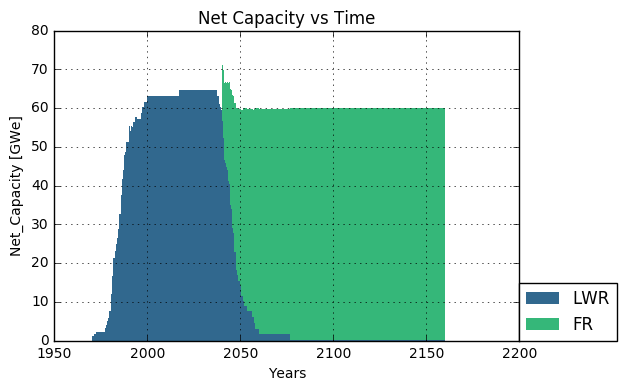
\includegraphics[width=\columnwidth]{./images/french-transition/number_plot.png}
	\end{center}
	\caption{French Transition into an SFR Fleet}
	\label{fig:sfr_num}
\end{figure}
\FloatBarrier


\Cref{fig:sfr_num} displays
the French transition into \glspl{SFR} over time.
The steep transition from 2035 to 2060 is due mainly to
French aggressive growth from 1975 to 2000. Note the jump in
2040 is due to an attempt to make up for the gap between the
mass decommission of old \glspl{LWR} and the availability
of \glspl{SFR}.

\subsection{Depletion Calculations}
Depletion calculations of the nuclear fuel are recipe-based, such that a fresh 
and used fuel recipe is used for each reactor type.
For the compositions of the fuel, a reference depletion calculation
from ORIGEN is used (see \cref{tab:comp}). The recipe has also been used for
\cite{wilson_adoption_2009}.

\subsection{Scenario Descriptions}
The simulation follows the model fuel cycle, where a `source'
provides natural uranium, which is enriched by an 'enrichment'
facility to produce \gls{UOX}, while disposing enrichment waste (tailings)
to the 'sink' facility. The enriched \gls{UOX} is used
in the \gls{LWR}s and \gls{UOX} waste is produced. The used fuel
is then reprocessed to separate plutonium and uranium.
The plutonium is mixed with depleted uranium (tailings) to \gls{MOX}.
The reprocessed uranium is stockpiled. The cycle is illustrated in
\cref{diag:fc}.

The second scenario separates plutonium from the \gls{UNF}
inventory from the previous simulation. The separated
plutonium is mixed with the depleted uranium inventory from the previous simulation
to create \gls{MOX}, which is used in the \gls{SFR}s. The used
\gls{MOX} is also reprocessed to extract plutonium, which is also
mixed with depleted uranium to produce \gls{MOX}.

